This lecture aims to look at periodic potentials and find the most general information we can about their energy spectrum. In order to do this we will use so-called \emph{Rigged Hilbert Spaces}.\footnote{I am currently reading up on these, and will add an additional section to the end of these notes once I have a better idea on them.}

\bd 
The Hamiltonian for a periodic potential is of the form 
\bse 
H = -\frac{\hbar^2}{2m} \Laplace + V(x),
\ese 
with 
\ben[label=(\roman*)]
\item Periodicity in $V(x)$, i.e. $V(x+a) = V(x)$ for all $x\in\R^3$ where $a$ is the periodicity of the system
\item $V$ is pointwise continuous and bounded.
\een 
\ed 

\begin{center}
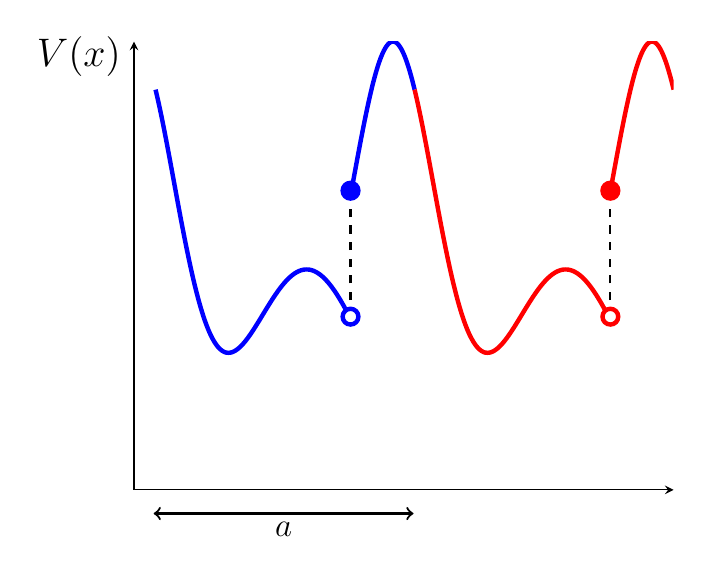
\begin{tikzpicture}
\begin{axis}[ticks=none,axis lines=middle]
    \addplot [domain=0.5:5, samples=100, ultra thick, blue] {6*exp((-x*x)/2) + 3*exp((-(x-4)^2)/4) + exp((-(x-10)^2)/6) + 3*exp((-(x+4)^2)/4) + exp((-(x+10)^2)/6)};
    \addplot [domain=5:6.5, samples=100, ultra thick, blue] {6*exp((-(x-6)^2)/2) + 3*exp((-(x-10)^2)/4) + exp((-(x-16)^2)/6) + 3*exp((-(x-2)^2)/4) + exp((-(x+4)^2)/6)};
    \addplot [domain=6.5:11, samples=100, ultra thick, red] {6*exp((-(x-6)^2)/2) + 3*exp((-(x-10)^2)/4) + exp((-(x-16)^2)/6) + 3*exp((-(x-2)^2)/4) + exp((-(x+4)^2)/6)};
    \addplot [domain=11:12.5, samples=100, ultra thick, red] {6*exp((-(x-12)^2)/2) + 3*exp((-(x-16)^2)/4) + exp((-(x-22)^2)/6) + 3*exp((-(x-8)^2)/4) + exp((-(x-2)^2)/6)};
    \addplot[domain=0:1]{0};
\end{axis}
\draw[dashed, thick] (2.75,2.2) -- (2.75,3.8);
\draw[blue, ultra thick, fill=white] (2.75,2.2) circle [radius=0.1];
\draw[blue, ultra thick, fill=blue] (2.75,3.8) circle [radius=0.1];
\draw[dashed, thick] (6.05,2.2) -- (6.05,3.8);
\draw[red, ultra thick, fill=white] (6.05,2.2) circle [radius=0.1];
\draw[red, ultra thick, fill=red] (6.05,3.8) circle [radius=0.1];
\node at (6.8,-0.3) {\Large{$\R$}};
\node at (-0.7,5.5) {\Large{$V(x)$}};
\draw[<->, thick] (0.25,-0.3) -- (3.55,-0.3);
\node at (1.9,-0.5) {\large{$a$}};
\end{tikzpicture}
\end{center}

As we shall see, by making no assumptions apart from the above, we will be able to extract a remarkable generic conclusion about the energy spectrum of particle moving in a generic periodic potential. This is truly a amazing result as the potential can even be discontinuous (countably) infinite times! A huge application of this formalism is in the study of solid state physics, where the periodic potential comes from that generated by a regular lattice of so-called \emph{lattice constant} $a$, 

\begin{center}
    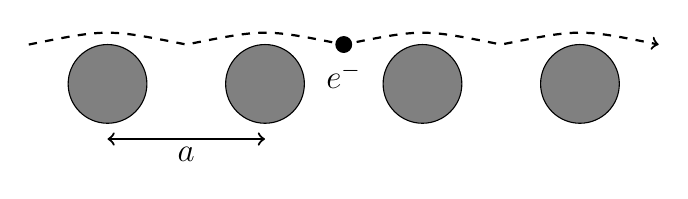
\begin{tikzpicture}
    \draw[fill=gray] (0,0) circle [radius=0.5];
    \draw[fill=gray] (2,0) circle [radius=0.5];
    \draw[fill=gray] (4,0) circle [radius=0.5];
    \draw[fill=gray] (6,0) circle [radius=0.5];
    \draw[<->, thick] (0,-0.7) -- (2,-0.7); 
    \node at (1,-0.9) {\large{$a$}};
    \draw[fill=black] (3,0.5) circle [radius=0.1];
    \node at (3,0.1) {\large{$e^-$}};
    \draw[->, thick, dashed] (-1, 0.5) .. controls (0,0.7) .. (1,0.5) .. controls (2,0.7) .. (3,0.5) .. controls (4,0.7) .. (5,0.5) .. controls (6,0.7) .. (7,0.5);
    \end{tikzpicture}
\end{center}

As we shall see the general result is that the energy spectrum comes in continuous, open intervals in $\R$, known as \emph{bands}.

\begin{center}
    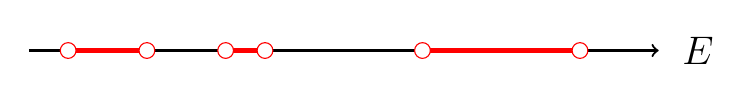
\begin{tikzpicture}
    \draw[thick, ->] (0,0) -- (8,0);
    \node at (8.5,0) {\Large{$E$}};
    \draw[ultra thick, red] (0.5,0) -- (1.5,0);
    \draw[red, fill=white] (0.5,0) circle [radius=0.1];
    \draw[red, fill=white] (1.5,0) circle [radius=0.1];
    \draw[ultra thick, red] (2.5,0) -- (3,0);
    \draw[red, fill=white] (2.5,0) circle [radius=0.1];
    \draw[red, fill=white] (3,0) circle [radius=0.1]; 
    \draw[ultra thick, red] (5,0) -- (7,0);
    \draw[red, fill=white] (5,0) circle [radius=0.1];
    \draw[red, fill=white] (7,0) circle [radius=0.1];
    \end{tikzpicture}
\end{center}

\subsection{Basics of Rigged Hilbert Space}

As mentioned at the start, we wish to make use of rigged Hilbert spaces\footnote{Again, coming soon!} in order to find the spectrum of the energy observable. The basic reason behind this is that rigged Hilbert spaces essentially extend what we usually think of as the eigenvalue equation
\bse 
H\psi = E\psi, 
\ese 
where $E$ is a discrete value in $\R$, to the case where $E$ can be continuous. This is known as the \emph{generalised eigenvalue equation}.

We do this because ultimately we know that the spectrum will be continuous intervals, however even if it was purely discrete, or a combination of both, the theory of rigged Hilbert spaces would still account for this. 

The basic idea behind rigged Hilbert spaces is to consider elements $\Psi$ that satisfy the generalised eigenvalue equation, but do not lie in $L^2(\R^d)$. It turns out that they lie in the adjoint of a densely defined subspace, which for us is the Schwartz space. In this way we construct our so-called \emph{Gelfand Triple}:
\bse 
S(\R^d) \ss L^2(\R^d) \ss S^*(\R^d).
\ese 

The easiest way to see that we need such a construction here is that, as the Hamiltonian is constructed using derivative operators, its eigenvalues are likely to be of the form 
\bse 
\Psi \propto e^{iE},
\ese
which is clearly not square integrable (it's modulus is 1).

\br 
It is important to note here that a rigged Hilbert space is not some extension of the physics or of quantum mechanics, but indeed it is the most natural mathematical structure required in order to study quantum mechanics. In fact it is the rigged Hilbert space structure which provides the full mathematical foundation in order to understand Dirac's bra-ket notation, and it introduces the well known \emph{Dirac delta function}. This gives the first insight into what a rigged Hilbert space is --- it is the equipping (i.e. the `rigging') of a Hilbert space with a theory of distributions. 
\er 

\bp
Any $H$-eigenvector $\Psi\in S*(\R^d)\setminus L^2(\R^d)$ has a purely continuous energy spectrum.
\ep 

\subsection{Fundamental Solutions and Fundamental Matrix}

\bd 
A set of solutions $\{\psi_1,...,\psi_n\}$ for a system of linear, homogeneous ordinary differential operators is known as a \emph{fundamental set of solutions} if 
\ben[label=(\roman*)]
\item They are linearly independent 
\item Any other solution to the ODEs can be expanded using the set $\{\psi_1,...,\psi_n\}$.
\een 

In other words, they form a basis for the solution space. 
\ed 

\bp 
The cardinality of the fundamental set of solutions of a system of $n$-th order ODEs is $n$.
\ep 

\be 
Let the system of ODEs just be the single equation 
\bse 
\ddot{\psi}(x) + \omega^2\psi(x) = 0,
\ese 
for some non-vanishing $\omega\in\R$. The the fundamental set of solutions is 
\bse 
\psi_1 = \cos(\omega x) \qquad \text{and} \qquad \psi_2 = \sin(\omega x).
\ese 
It is easy enough to see that these two solutions do indeed form a basis for the solution space.
\ee 

\bl 
Let $\{\psi_1,...,\psi_n\}$ be a set of fundamental solutions for some system of ODEs. Then the set $\{c_1\psi_1,...,c_n\psi_n\}$ for $c_i\in\F$ (the underlying field) is also a set of fundamental solutions. 
\el 

As our Hamiltonian is a second order ODE there are 2 fundamental solutions. These fundamental solutions depend on the value of $E$ and so we label them as $\{\psi_1^E,\psi_2^E\}$. We remove the ambiguity in the coefficients by requiring 
\bi{rCl}
\psi_1^E(0) = 1, & \qquad & (\psi_1^E)'(0) = 0 \\
\psi_2^E(0) = 0, & \qquad & (\psi_2^E)'(0) = 1.
\ei 

\bd 
An \emph{entire function} is a complex valued function that is holomorphic ($\C$-differentiable in the neighbourhood of a point) at all finite points in the complex domain.
\ed 

\bt 
The fundamental solutions $\psi_1^E$ and $\psi_2^E$ are entire functions on $E$. 
\et 

\br 
Note in order to make the above theorem true, we require that our eigenvalues are complex, $E\in\C$. This is clearly unphysical, however do this here in order to exploit the strong results of complex analysis, and then we shall restrict ourselves to $E\in\R$ at the end. 
\er 

\bd 
The \emph{fundamental matrix} of a system of linear, homogeneous ODEs, with the fundamental set of solutions $\{\psi_1,...,\psi_n\}$ is the matrix 
\bse 
M(x) = \begin{pmatrix}
\psi_1(x) & ... & \psi_n(x) \\
\psi_1'(x) & ... & \psi_n'(x) \\
. & ... & . \\
. & ... & . \\
. & ... & . \\
\psi_1^{(n)}(x) & ... & \psi_n^{(n)}(x)
\end{pmatrix}
\ese 
\ed 

\bl 
The determinant fundamental matrix for our system is constant\footnote{Note we also label $M$ with a superscript $E$.}
\bse 
\big[\det M^E\big]'(x) = 0.
\ese 
\el 

\bq 
By direct calculation, and using the generalised eigenvalue equation, 
\bi{rCl}
\big[ \psi_1^E(\psi_2^E)' - (\psi_1^E)'\psi_2^E \big]'(x) & = & \big[ (\psi_1^E)'(\psi_2^E)'  + \psi_1^E(\psi_2^E)'' -  (\psi_2^E)'(\psi_1^E)' - (\psi_1^E)''\psi_2^E \big](x) \\
& = & \bigg[ \psi_1^E\bigg(-\frac{2m}{\hbar^2}(E-V)\psi_2^E\bigg) - \bigg(-\frac{2m}{\hbar^2}(E-V)\psi_1^E\bigg)\psi_1^E\bigg](x) \\
& = & 0.
\ei 
\eq 

\bc 
It follows trivially from the conditions we placed on $\psi_1^E$ and $\psi_2^E$ that $\det M^E(x) =1$.
\ec 

\subsection{Translation Operator}

\bd 
The \emph{translation operator} is the linear operator such that its action on an element in its domain is given by 
\bse 
(T\psi)(x) := \widetilde{\psi}(x) := \psi(x+a),
\ese 
for some $a\in\C$. 
\ed 

\bp 
Let $T$ be the translation operator with $a$ being the periodicity of our system. Then the $T$ commutes with the Hamiltonian, 
\bse 
[T,H] = 0.
\ese 
\ep 

\bq 
Consider the action on an element $\psi$ in the codomain of both operators, 
\bi{rCl}
[T,H]\psi(x) & = & T(H\psi)(x) - H(T\psi)(x) \\
& = & T \bigg(-\frac{\hbar^2}{2m}\Laplace \psi + V \psi\bigg)(x) - H(T\psi)(x) \\
& = & \bigg(-\frac{\hbar^2}{2m} \Laplace T\psi + V T\psi\bigg)(x) - H(\widetilde{\psi})(x) \\
& = & H(T\psi)(x) - H(T\psi)(x) \\
& = & 0,
\ei
where we have used the fact that the translation by a constant doesn't effect the result of differentiating a function and the fact that $T$ is linear. 
\eq 

\bl 
Let $\psi^E$ be a $H$-eigenvector of our system. Then $\widetilde{\psi}^E := T\psi^E$ is also a $H$-eigenvector.
\el 

\bq 
From the commutation result, 
\bi{rCl}
H(T\psi^E)(x) & = & T(H\psi^E)(x) \\
H\widetilde{\psi}^E(x) & = &  T (E\psi^E)(x) \\
& = & E(T\psi^E)(x) \\
& = & E \widetilde{\psi^E}(x).
\ei 
\eq 

So we have that the translated solution is also a solution. We now use the fact that $\{\psi_1^E,\psi_2^E\}$ is a fundamental set of solutions to expand the translated fundamental solution,  
\bse 
\psi_j^E(x+a) = \sum_{i=1}^2 {a^i}_j \psi_i^E(x),
\ese 
for $j=1,2$.

Now consider the case for $x=0$, then we have 
\bi{rCl}
\psi_j^E(a) & = & {a^1}_j\psi_1^E(0) + {a^2}_j\psi_2^E(0) \\
& = & {a^1}_j,
\ei 
and similarly 
\bse 
(\psi_j^E)'(a) = {a^2}_j,
\ese 
from which it follows that 
\bse 
{a^i}_j = {\big(M^E(a)\big)^i}_j.
\ese 

So we have that a general solution is of the form 
\bse 
\psi^E(x+a) = \sum_{\ell=1}^2 \sum_{i=1}^2 A^{\ell} {\big(M^E(a)\big)^i}_j \psi_i^E(x),
\ese 
for $A^1,A^2\in\C$.

\br 
As we showed previously the translation operator and the Hamiltonian commute, and so they share common eigenvectors. We shall label these eigenvectors as follows \bi{rCl}
H\psi^{E,\lambda} & = & E\psi^{E,\lambda}, \\
T \psi^{E,\lambda} & = & \lambda \psi^{E,\lambda}.
\ei 
\er 

We can reformulate the second eigenvalue equation as follows: using $T\psi^{E,\lambda}(x) = \psi^{E,\lambda}(x+a)$ we have
\bi{rCl}
\psi^{E,\lambda}(x+a) & = & \lambda \psi^{E,\lambda}(x) \\
\sum_{\ell=1}^2\sum_{i=1}^2 A^{\ell}_{\lambda} {\big(M^E(a)\big)^i}_{\ell} \psi^E_i(x) & = &  \lambda \sum_{i=1}^2 A^i_{\lambda} \psi^E_i(x),
\ei 
where we have introduced a $\lambda$ label (not an index!) on $A$ to indicate that it corresponds to a specific $\lambda$. Now using the linear independence of the fundamental solutions, we can equate coefficients, then noting that the LHS is just matrix multiplication we see that we can write $A_{\lambda}$ as a column matrix with two entries 
\bse 
A_{\lambda} = \begin{pmatrix}
A_{\lambda}^1 \\
A_{\lambda}^2
\end{pmatrix},
\ese 
which is an eigenvalue of the fundamental matrix at $a$ with eigenvalue $\lambda$. 

If we let $\lambda_1$ and $\lambda_2$ be the two eigenvalues of $M^E(a)$, then there is some basis such that 
\bse 
M^E(a) = \begin{pmatrix}
\lambda_1 & 0 \\
0 & \lambda_2
\end{pmatrix},
\ese 
from which we have\footnote{Note these results are basis independent for any transformation given by an endomorphism.} 
\bi{rCl}
\det M^E(a) & = & \lambda_1\cdot \lambda_2 \\
\Tr M^E(a) & = & \lambda_1 + \lambda_2.
\ei 

Then using the result $\det M^E(a)=1$, we have the condition
\bse 
\lambda_1 = \frac{1}{\lambda_2},
\ese 
and we just want some way to find the trace to work out what the second condition is. 

\subsection{Application to Our Quantum Problem}

\bt[Floquet\footnote{Based on a combination of the one given in the lectures and the one given on \href{http://mathworld.wolfram.com/FloquetsTheorem.html}{Wolfram}.}]
Let $V(x)$ be a complex, piecewise continuous, periodic function with minimum period $\pi$. Then the solutions to the ODE
\bse 
y'' + V(x)y = 0
\ese 
are linearly independent and can be written as 
\bi{rCl}
f_1(x) & = & e^{i\theta x} p_1(x) \\
f_2(x) & = & e^{-i\theta x} p_2(x),
\ei 
for $\theta \in [-\pi,\pi)$ and where $p_1(x)$ and $p_2(x)$ are periodic with the same period as $V(x)$.
\et 

\br 
Floquet's theorem also tells us that the eigenvalues are simply 
\bse 
\lambda_1 = e^{i\theta} \quad \text{and} \quad \lambda_2 = e^{-i\theta}.
\ese 
\er 

We have, then, that 
\bse 
\psi^E_1(a) + \psi^E_2(a) = \Tr M^E(a) = e^{i\theta} + e^{-i\theta} = 2\cos\theta.
\ese 
We now define the function 
\bse 
\gamma_V(E) := \frac{1}{2} \big(\psi^E_1(a) + \psi^E_2(a) \big) = \cos\theta,
\ese 
where the subscript indicates that its for the type of potentials we're considering.

\subsection{Energy Bands}

Recall that $\psi^E_1$ and $\psi^E_2$ are entire functions of $E$, and so their sum is also an entire function. From this it follows that the restriction of $\gamma_V$ to the reals, 
\bse 
\gamma_V|_{\R} : \R \to \C,
\ese 
is at least smooth. Thus we know that 
\ben[label=(\roman*)]
\item If $(E_0,\theta_0)$ solves the equation $\gamma_V(E_0) = \cos\theta_0$, then any $E$ in a sufficiently small neighbourhood of $E_0$ solves the equation $\gamma_V(E) =\cos\theta$ for some $\theta$. 
\item Equivalently, if $E_1$ does \emph{not} solve $\gamma_V(E_1)=\cos(\theta_1)$ for \emph{any} $\theta_1\in([\pi,\pi)$, then no $E$ is any sufficiently small neighbourhood will. 
\een 

From these conditions we can draw the remarkable conclusion: For any periodic, piecewise continuous and bounded potential, the energy spectrum is a countable union of open intervals, known as energy bands. 

\br 
Note the fact that we only have continuous parts to our spectrum is consistent with our rigged Hilbert space ideas; the functions $\psi^{E,\lambda}$ contain a phase factor and then a periodic function, and so are not square integrable, but they are bounded and so are elements of $S^*(\R^d)\setminus L^2(\R^d)$.
\er 

\subsection{Quantitative Calculation (Outline)}

To obtain the precise intervals (bands) one needs to find (perhaps numerically) the fundamental solutions. One obtains, for instance, for a potential of the form 

\begin{center}
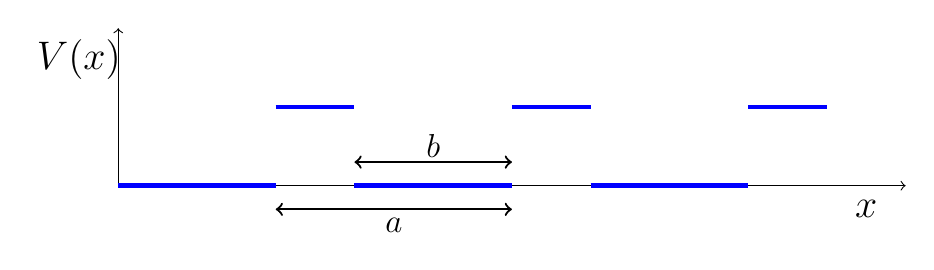
\begin{tikzpicture}
\draw[->] (0,0) -- (10,0);
\draw[->] (0,0) -- (0,2);
\draw[ultra thick, blue] (0,0) -- (2,0);
\draw[ultra thick, blue] (2,1) -- (3,1);
\draw[ultra thick, blue] (3,0) -- (5,0);
\draw[ultra thick, blue] (5,1) -- (6,1);
\draw[ultra thick, blue] (6,0) -- (8,0);
\draw[ultra thick, blue] (8,1) -- (9,1);
\draw[thick, <->] (2,-0.3) -- (5,-0.3);
\draw[thick, <->] (3,0.3) -- (5,0.3);
\node at (3.5, -0.5) {\large{$a$}};
\node at (4, 0.5) {\large{$b$}};
\node at (-0.5, 1.6) {\Large{$V(x)$}};
\node at (9.5, -0.3) {\Large{$x$}};
\end{tikzpicture}
\end{center}
results in energy bands of the form

\begin{center}
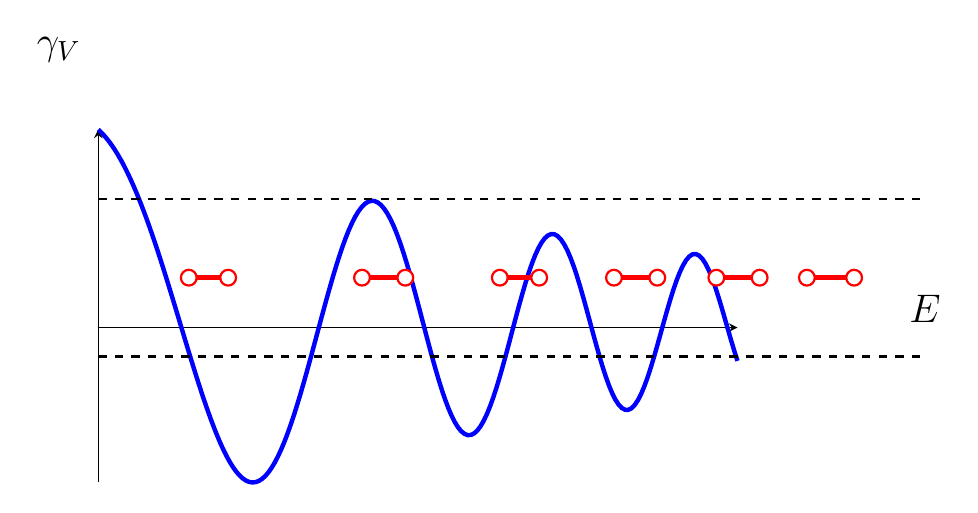
\begin{tikzpicture}
  \begin{axis}[
    trig format plots=rad,
    axis lines = middle,
    clip=false,
    ticks=none, 
    width=0.8\textwidth,
    height=0.5\textwidth
    ]
    \addplot[domain=0.42:1.5,samples=200,blue, ultra thick] {4*exp(-x)*sin(10*x^2)};
  \end{axis}
  \draw[thick, dashed] (0,3.6) -- (10.5,3.6); 
  \draw[thick, dashed] (0,1.6) -- (10.5,1.6);
  \draw[ultra thick, red] (1.15,2.6) -- (1.65,2.6);
  \draw[red, fill=white, thick] (1.15,2.6) circle [radius=0.1];
  \draw[red, fill=white, thick] (1.65,2.6) circle [radius=0.1];
  \draw[ultra thick, red] (3.35,2.6) -- (3.9,2.6);
  \draw[red, fill=white, thick] (3.35,2.6) circle [radius=0.1];
  \draw[red, fill=white, thick] (3.9,2.6) circle [radius=0.1];
  \draw[ultra thick, red] (5.1,2.6) -- (5.6,2.6);
  \draw[red, fill=white, thick] (5.1,2.6) circle [radius=0.1];
  \draw[red, fill=white, thick] (5.6,2.6) circle [radius=0.1];
  \draw[ultra thick, red] (6.55,2.6) -- (7.1,2.6);
  \draw[red, fill=white, thick] (6.55,2.6) circle [radius=0.1];
  \draw[red, fill=white, thick] (7.1,2.6) circle [radius=0.1];
  \draw[ultra thick, red] (7.85,2.6) -- (8.4,2.6);
  \draw[red, fill=white, thick] (7.85,2.6) circle [radius=0.1];
  \draw[red, fill=white, thick] (8.4,2.6) circle [radius=0.1];
  \draw[ultra thick, red] (9,2.6) -- (9.6,2.6);
  \draw[red, fill=white, thick] (9,2.6) circle [radius=0.1];
  \draw[red, fill=white, thick] (9.6,2.6) circle [radius=0.1];
  \node at (-0.5,5.5) {\Large{$\gamma_V$}};
  \node at (10.5,2.2) {\Large{$E$}};
\end{tikzpicture}
\end{center}